% !TEX root = LMThesisNicchi.tex

\chapter{Background} \label{background}

In literature there are many different implementations of API hooking. The objective of this chapter is to provide an outline of the various approaches utilized to hook functions in DLLs, outlining the benefits and the limitations of each technique, with a strong focus on their detection by malicious software. In particular, the focus will be on user space API hooking of \texttt{Win32} binaries, since this is BlueTracer's current field of application. Obviously, as it is the norm in malware analysis, it also assumed that the program under study is only available in binary form.

Depending on their underlying implementation, API hooking techniques can be divided in three broad categories: \textbf{Binary Rewriting}, \textbf{Virtul Machine Introspection (VMI)} and \textbf{Dynamic Binary Instrumentation (DBI)}.   

\section{Binary Rewriting}

Binary rewriting-based hooking involves inserting hooks at the API entries, via one of the following two approaches:
\begin{enumerate}
\item Redirecting all \texttt{call} instructions so that the hook is called instead of the original function.
\item Rewriting the function of interest such that, before its invocation, the hook is executed. 
\end{enumerate} 

In both cases the hook function gains access to all the arguments present on the stack, thus being able to carry out all the required analysis operations.

The main techniques which use the first approach are \textit{Import Address Table (IAT) Patching}, \textit{Export Address Table (EAT) patching} and \textit{Proxy DLL}. On the other hand, the most significant techniques which use the second approach are \textit{inline hooking} and \textit{debugger-based hooking} (\textit{Figure~\ref{HookTech}}).



\begin{figure}[h]
\centering
\hspace*{-3em}
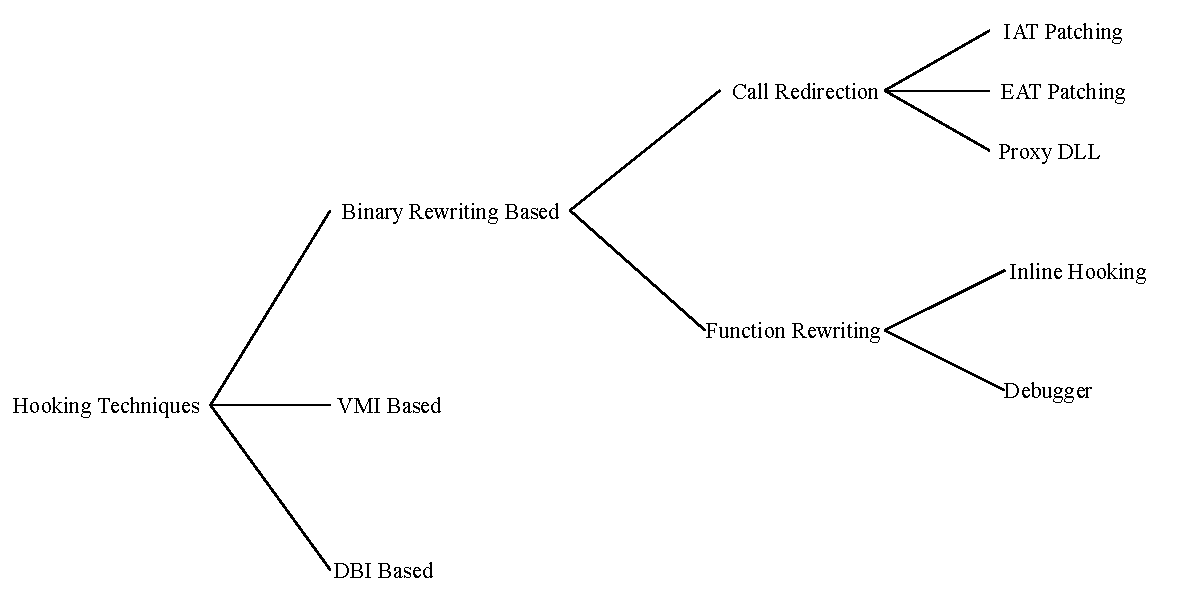
\includegraphics[scale=0.8]{Figures/API-hooking-3.pdf}
\caption{\textit{API hooking techniques classification}}
\label{HookTech}
\end{figure}

\subsection{Import Address Table Patching}

In the header of every Portable Executable (PE) file there is an Import Address Table (IAT) for every dynamic-link library (DLL) that is included by the executable \cite{Berdajs:2010:EAU:1815744.1815746} (\textit{Figure~\ref{IAT}}). This table is utilized to indicate the location of DLL-imported functions in virtual memory and is filled by the Windows loader with the actual function memory addresses after the executable is loaded in memory.

\begin{figure}[h]
\centering
\hspace*{-3em}
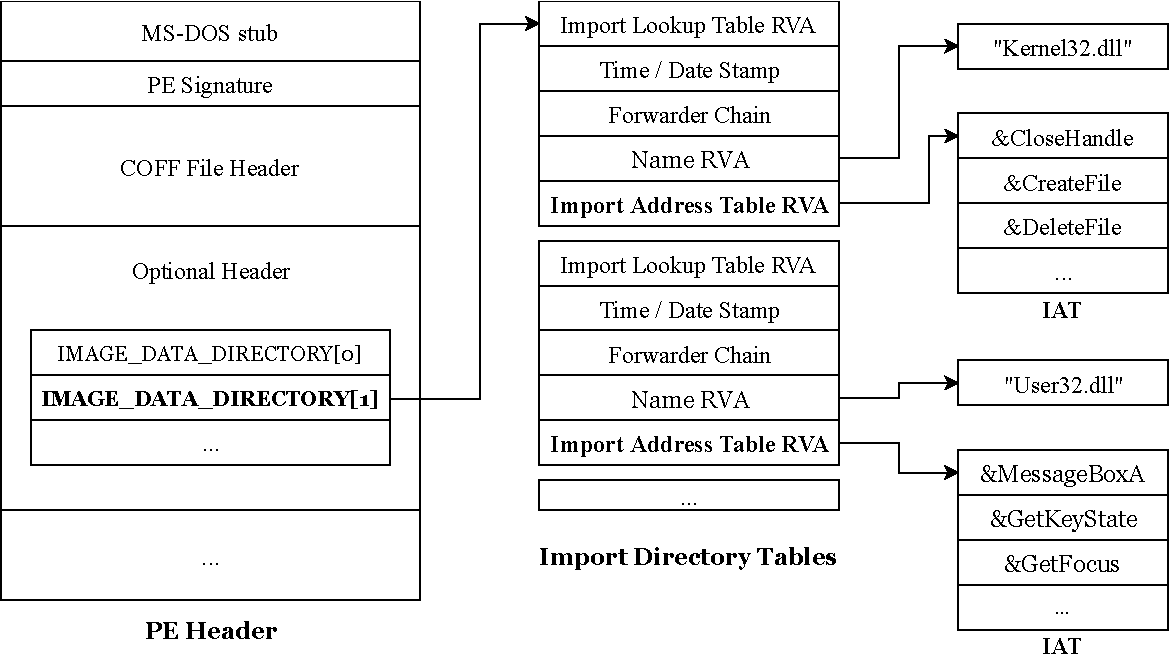
\includegraphics[scale=0.8]{Figures/IAT-3.pdf}
\caption{\textit{IAT in PE header}}
\label{IAT}
\end{figure}

The idea is to overwrite the original pointer to an imported API function so that, instead of pointing to the original API, it will point to a different function.

\newpage

Despite being extremely simple to implement, IAT patching suffers from a couple of disadvantages, which significantly limit its use in practice:
\begin{itemize}
    \item It is incredibly easy to detect by simply examining the entries of the IAT and checking whether or not each address falls inside the memory range of the DLL that should contain the function \cite{HookingDetection}.
    \item It is ineffective when function pointers are acquired dynamically, e.g., via \texttt{LoadLibrary} and \texttt{GetProcAddress} \cite{Buescher:2011:BIS:2186328.2186347}.
\end{itemize}

\subsection{Export Address Table Patching}

Export Address Table (EAT) patching is similar to IAT patching, with the difference that DLL export address tables are patched instead. The export address table (EAT) contains the name of every function exported by the DLL together with the relative virtual address (RVA) where the function can be found, which is relative to the DLL base address when loaded in memory. To hook an API function via EAT patching all that is needed is to overwrite the corresponding address in the table with the address of another function.

EAT patching produces similar results to the ones obtained through IAT patching, but, unlike IAT patching, the created hooks are global, i.e., they affect every program which utilizes the altered DLL \cite{Berdajs:2010:EAU:1815744.1815746}.

However, in a similar manner to what occurs for IAT patching, it can be easily detected by simply examining the entries of the EAT and checking whether or not each RVA, when added to the DLL base address, falls within the DLL memory range \cite{Stuttard:2014:ADC:2616217}.

\subsection{Proxy DLL}

In the Proxy DLL approach to hooking, also known as Trojan DLL, the DLL containing the functions to be hooked is replaced with another one having an identical name and exporting all the symbols of the original DLL \cite{CodeProjectHooking}. In addition to calling the original functions so that they can carry out their tasks, the Proxy DLL may also make available different implementations for the hooked functions \cite{Berdajs:2010:EAU:1815744.1815746}.

Even though a Proxy DLL is trivial to implement, it is also extremely easy to detect since the original DLL is substituted with another file, which is very likely to have a different size. Moreover, checksums could be employed to detect the presence of a Trojan DLL.


\subsection{Inline Hooking}

In \textit{inline hooking} the API to be hooked has its initial instructions (at least the first 5 bytes) overwritten with an unconditional jump to a replacement function. In order to ensure that the API's original functionality is not lost due to the modification of its entry point, a \textit{trampoline function} is created, consisting of a copy of the overwritten instructions and an unconditional jump back to the unaltered portion of the original function. As a result of this, the replacement function can invoke the original function by calling the trampoline, after performing all the desired analysis operations \cite{Berdajs:2010:EAU:1815744.1815746}.
\textit{Figure~\ref{Inlined}} illustrates a program's execution flow before and after the use of \textit{inline hooking}.

\begin{figure}[h]
\centering
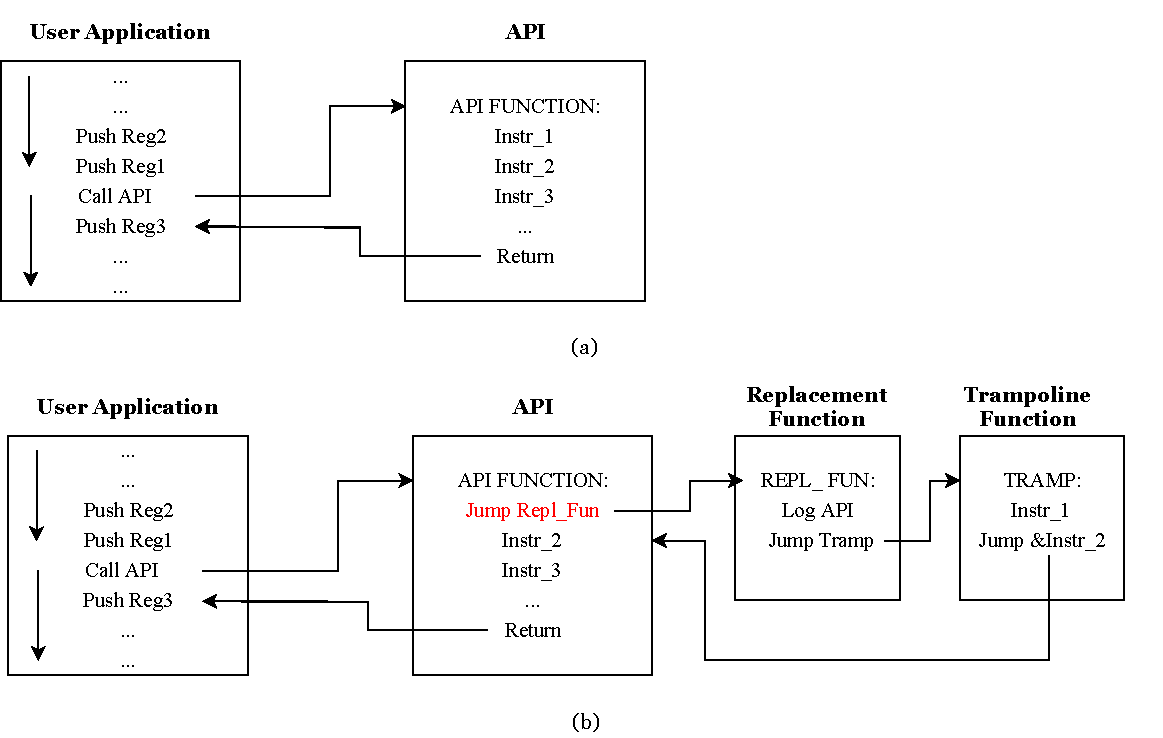
\includegraphics[scale=0.8]{Figures/Inline.pdf}
\caption{\textit{(a) Ordinary API call execution flow \\
				  (b) API call with inline hooking}}
\label{Inlined}
\end{figure}

\textit{Inline Hooking}, which was made famous by its employment  in the Microsoft \textit{Detours} Windows API hooking library, is one of the most used API hooking techniques since it offers a number of advantages:
\begin{itemize}
\item It is fast and efficient.
\item It can be utilized to hook any code, not just operating systems APIs, but also programmer defined functions \cite{Rootkit}. 
\item Unlike IAT patching, the type of command used to call the function does not matter, meaning that the hooking will be effective regardless of the fact that a function is called using the IAT or using \texttt{LoadLibrary} together with \texttt{GetProcAddress}.
\end{itemize} 

Unfortunately though, \textit{inline hooking} is also affected by some limitations:

\begin{itemize}
\item Can be easily detected, for instance by comparing the code section of system libraries in memory with a matching original copy loaded from the file system to detect library modifications \cite{Buescher:2011:BIS:2186328.2186347} or by searching API entry points for specific patterns (e.g., presence of \texttt{jmp} instructions) \cite{HookingDetection}.
\item It needs additional modifications in the case where the function's entry points includes specific instructions, like ones which contain relative memory addresses. In fact, such instructions cannot be executed from a trampoline as the trampoline is located in a different memory location than the one of the original program code \cite{Berdajs:2010:EAU:1815744.1815746}.
\end{itemize}

\subsection{Debugger-Based Hooking} \label{Debugger}

Hooking through the use of a debugger is realized by instructing the debugger to position a breakpoint at the entry point of the target API function. The placement of a breakpoint involves overwriting the initial instructions of the target API functions with CPU specific instructions, like \texttt{INT 3} for \texttt{IA-32}. These lead the CPU to throw a debug exception in case they are pointed by the current instruction pointer (IP). The exception is then intercepted by the debugger, which is able to deduce the API which is being called by the application from the address at which the exception took place \cite{HookingDetection}. Moreover, the debugger also has total control over the memory contents and the CPU state of the process being debugged.

Contrarily to inline hooking, a debugger can be used to hook functions whose entry points include instructions containing relative addresses \cite{Berdajs:2010:EAU:1815744.1815746}.

On the other hand, a debugger is much easier to detect. In fact, there exist specific Windows APIs whose purpose is to find out whether or not the current process is being debugged. For example, \texttt{IsDebuggerPresent} allows to determine if the calling process is running under a debugger, while \texttt{CheckRemoteDebuggerPresent} checks for the presence of a debugger in a separate process. 
In addition, the \texttt{INT 3} instruction in an API entry point immediately gives away the debugger's presence \cite{HookingDetection}.



\section{Virtual Machine Introspection}

Hooking based on Virtual Machine Introspection (VMI) relies on the idea of executing the target program in an emulated environment, typically with QEMU being used as virtual machine monitor (VMM). Function calls are monitored by comparing the virtual processor's instruction pointer with the RVAs of DLLs' exported functions when added to the DLL base address. Function arguments are also monitored and this is done by providing them to callback routines, which perform the appropriate tracking operations.

In theory, a PC emulator allows to have functionalities similar to the ones of a debugger, i.e., the code being monitored can be stopped at any arbitrary point during its execution, allowing its registers and virtual memory to be inspected, with the added advantage of not being subject to the aforementioned issues related to breakpoints.
Moreover, VMI-based hooking is harder to detect with respect to the previously illustrated hooking techniques, since emulation is utilized to execute an unknown binary with a complete operating system in software, without the sample being never ran directly on the processor \cite{Bayer2005TTAnalyzeA}.

The significant drawback of VMI-based hooking is that it incurs in the \textit{semantic gap} problem, i.e., the issue of deducing high-level information from the raw system information by making sense of the CPU state and memory contents \cite{Egele:2008:SAD:2089125.2089126}. VMI-based hooking tools
might need an in-depth knowledge of kernel data structures or other details at low-level, which could constitute a complication when dealing with proprietary operating systems. For this reason, as of right now, VMI is not as effective in practice as a traditional debugger when investigating a sample.


\section{Dynamic Binary Instrumentation} \label{DBI}

\iffalse
- Program analysis: source vs binary. As opposed to source analysis, in which ..., in binary analysis the idea is blablabla. The employed technique here is instrumentation.
- Instrumentation is blablabla. It can be either static or dynamic, where in both cases it is mandatory blablabla.
- Dynamic is better because blabla.
- Its main drawback is performance but recent frameworks blablabla
\fi

Instrumentation is commonly referred to as the act of adding extra analysis code to a program. There are two main instrumentation techniques being employed in dynamic binary analysis, where the main difference is constituted by when the instrumentation process takes place:

\begin{itemize}
\item \textit{Static Binary Instrumentation}, which takes place before the application is executed and involves the rewriting of object code or executable code.
\item \textit{Dynamic Binary Instrumentation} (DBI), 	which happens at run-time. The analysis code can be injected by a specific program attached to the target process or by an external process \cite{Nethercote2004CI}. 
\end{itemize}   

Dynamic Binary Instrumentation (DBI) is, therefore, a dynamic binary analysis technique in which the behavior of an application is inspected at run-time via the injection of analysis code. Such code, after being injected, executes as a component of the ordinary instruction flow, allowing to learn information about the behavior and the state of a sample at different points during its execution \cite{DBI}. Typically, DBI tools make use of a Just In Time (JIT) compiler to instrument the binary under analysis at run-time, the purpose of which is to translate \texttt{x86} code into an intermediate representation \cite{polino_arancino_2017}.

DBI, conversely from static binary instrumentation does not need any preprocessing of the program to be analyzed. This is what makes it more appealing for developers for profiling and tracing purposes. On top of that, DBI can be utilized for any program while static techniques are restricted in the code they can instrument, e.g., they cannot employed for code that is dynamically generated \cite{6658603}. The main drawback of DBI is that the instrumentation cost is encountered at run time, leading to performance degradation. However, in recent years, this issue has been mitigated by the introduction of generic DBI frameworks, which are accurately optimized to minimize the execution overhead \cite{Nethercote2004CI}.

In DBI-based hooking, the idea is to use DBI with the objective of learning information at run-time relative to which APIs are called by the sample being analyzed and, possibly, with which arguments and return values. 

There indeed exist DBI-based API tracing tools that rely on the previously illustrated idea, namely \textit{drstrace} and \textit{drltrace}, which are both built on top of the DynamoRIO \cite{DynamoRIO} DBI framework. In particular, \textit{drstrace} is a system call tracer for Windows, while \textit{drltrace} is an API calls tracer for both Windows and Linux applications. They both produce a textual log, in which the invoked APIs are recorded, together with their argument values and return values.

In order to evaluate the effectiveness of such tools in the context of evasive malware analysis, a series of experiments involving them was carried out. In particular, both tools were employed to analyze 1000 random samples from the Arancino\footnote{Arancino is a dynamic protection framework aimed at providing protection from anti-instrumentation attacks \cite{polino_arancino_2017}} dataset of malware samples (about 20\% of the total). Each malware sample was ran for 5 minutes in a VirtualBox environment with Windows 7 \texttt{x86} SP1 as the guest operating system. The analysis of the resulting logs showed that both tools possess critical shortcomings when analysing evasive malware. In particular: 

\begin{itemize}
\item They are not equipped with any mechanism aimed at cloaking the execution environment in order to prevent a malicious sample from detecting the DBI.
\item They are limited in the amount of information recorded relative to the traced APIs. This applies particularly to \textit{drltace}, which, unlike \textit{drstrace}, does not log return values and output values for arguments, in addition to not providing a mechanism for translating enumerations' constants to the appropriate name. Furthermore, both tools do not take into consideration Windows callbacks and asynchronous procedure calls (APC).
\end{itemize}

This highlights how the current DBI-based methods are lacking when having to deal with the dynamic analysis of evasive malware and that there is much room for improvement in this area.

\section{Conclusion}

In this chapter we showed how the state of the art API hooking techniques suffer from a number of remarkable shortcomings, especially when dealing with evasive malware. In fact, binary rewriting-based hooking techniques are all easily detectable, while VMI, although harder to uncover, is affected by the \textit{semantic gap problem}. Finally, existing DBI-based API tracing tools are not accompanied by adequate cloaking mechanisms and are limited in the amount of logged information. The aforementioned issues indicate that there is a need for a robust API tracer, specialized in the analysis of evasive malware and with extensive logging capabilities. This is the rationale at the heart of BlueTracer. 